\section{Simulation Testbed}
\label{sec:exp}

This section details our experimental settings in terms of the hardware
parameters, the database and query workload, and the performance metrics
on which we evaluated the PCM-conscious operator implementations.



\subsection{Architectural Platform}
Since PCM memory is as yet not commercially available, we
have taken recourse to a simulated hardware environment to
evaluate the impact of the PCM-conscious operators.  For this
purpose, we chose Multi2sim~\cite{multi2sim}, an open-source
application-only\footnote{Simulates only the application layer without
the OS stack.} simulator that can model a multithreaded, multicore,
superscalar x86 CPU and an AMD Evergreen GPU. It has support for both
functional simulation and cycle-accurate detailed architecture simulation.

We evaluated the PCM-conscious algorithms on Multi2sim in cycle-accurate simulation
mode. Since it does not have native support for PCM, we made a major
extension to its existing memory module to model PCM with a hardware-controlled DRAM buffer as main memory. Furthermore, we added separate data tracking functionality
for the DRAM and PCM-resident data, to implement the DCW scheme of DRAM line writeback to PCM discussed in Section \ref{sec:framework}. Likewise, we made several other enhancements to Multi2sim for PCM modelling, and these are exhaustively covered in \cite{techreport}.

\begin{center}
\begin{table}[t]
\begin{small}
\caption{Experimental Setup}
\label{table:setup}
\begin{tabular}{p{3cm}p{9cm}}
\toprule
Simulator & Multi2sim-4.2 with added support for PCM\\ \hline

L1D cache (private) & 32KB, 64B line, 4-way set-associative, 4 cycle latency, write-back, LRU\\ \hline
L1I cache (private) & 32KB, 64B line, 4-way set-associative, 4 cycle latency, write-back, LRU\\ \hline   
L2 cache (private) & 256KB, 64B line, 4-way set-associative, 11 cycle latency, write-back, LRU\\ \hline

DRAM buffer (private) & 4MB, 256B line, 8-way set-associative, 200 cycle latency, write-back, N-Chance (N = 4)\\ \hline

Main Memory & 2GB PCM, 4KB page, 1024 cycle read latency (per 256B line), 64 cycle write latency (per 4B modified word)\\ \bottomrule
\end{tabular}
\end{small}
\end{table}
\end{center}

\vspace{-0.4in}
The specific configurations used in the memory hierarchy \emph{(L1 Data,
L1 Instruction, L2, DRAM Buffer, PCM)} evaluated in our experiments are
enumerated in Table~\ref{table:setup}.  These values are scaled down
versions, wrt number of lines, of the hardware simulation parameters used
in \cite{wear} -- the reason for the scaling-down is to ensure that the
simulator running times are not impractically long. However, we have been
careful to ensure that the \emph{ratios} between the sizes of adjacent
levels in the hierarchy are maintained as per the original configurations
in \cite{wear}.  

%\vspace*{0.05in}

\subsection{Database and Queries}
%We used TPC-H (version 2.16.0) 1GB PCM-resident database for our experiments.
For the data, we used the default 1GB database generated by the TPC-H
benchmark.  This size is certainly small compared to the database sizes
typically encountered in modern applications -- however, we again chose
this reduced value to ensure viable simulation running times. Nevertheless, this database is significantly larger than the simulated DRAM (4MB), a faithful representation of most real-world scenarios.

For simulating our suite of database operators -- \textit{sort},
\textit{hash join} and \textit{group by} -- we created a separate library
consisting of the native PostgreSQL implementation of these operators. To
this library, we added the PCM-conscious versions described in the
previous sections.

While we experimented with several of the TPC-H queries, results for
three queries: Query 13 (Q13), Query 16 (Q16) and Query 19 (Q19), that
cover a diverse spectrum of the experimental space, are presented here.
For each of the queries, we first identified the query execution plan
recommended by the PostgreSQL query optimizer with the native operators,
and then forcibly used the same execution plan for their PCM-conscious
replacements as well. This was done in order to maintain fairness in the
comparison of the PCM-oblivious and PCM-conscious algorithms, though it
is possible that a better plan is available -- we return to this issue 
later in Section~\ref{discussion}. 

The execution plans associated with the three queries are shown in Figure~\ref{fig:plan_trees}. 
 


\begin{figure*}[t]
\centering
\subfloat[Q13]{
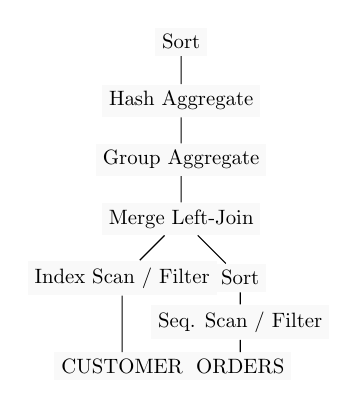
\begin{tikzpicture}[scale=.75, transform shape]

\tikzstyle{every node} = [rectangle, fill=gray!5]

\node (d) at (0,3) {Index Scan / Filter};
\node (c) at (0,1.5) {CUSTOMER};

\node (s) at (2,3) {Sort};
\node (p) at (2,2.25) {Seq. Scan / Filter};
\node (a) at (2,1.5) {ORDERS};

\node (e) at (1,4) {Merge Left-Join};
\node (f) at (1,5)  {Group Aggregate};
\node (g) at (1,6)  {Hash Aggregate};
\node (h) at (1,7)  {Sort};


\draw[-] (c) -- (d);
\draw[-] (a) -- (p);
\draw[-] (d) -- (e);
\draw[-] (p) -- (s);
\draw[-] (s) -- (e);
\draw[-] (e) -- (f);

\draw[-] (f) -- (g);
\draw[-] (g) -- (h);

\end{tikzpicture}
}
\subfloat[Q16]{
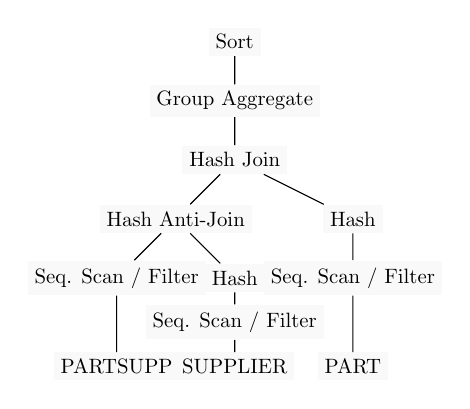
\begin{tikzpicture}[scale=.75, transform shape]

\tikzstyle{every node} = [rectangle, fill=gray!5]

\node (d) at (0,3) {Seq. Scan / Filter};
\node (c) at (0,1.5) {PARTSUPP};

\node (s) at (2,3) {Hash};
\node (p) at (2,2.25) {Seq. Scan / Filter};
\node (a) at (2,1.5) {SUPPLIER};

\node (e) at (1,4) {Hash Anti-Join};

\node (n) at (4, 4) {Hash};
\node (b) at (4,3) {Seq. Scan / Filter};
\node (x) at (4,1.5) {PART};

\node (f) at (2,5)  {Hash Join};
\node (g) at (2,6)  {Group Aggregate};
\node (h) at (2,7)  {Sort};


\draw[-] (c) -- (d);
\draw[-] (a) -- (p);
\draw[-] (d) -- (e);
\draw[-] (p) -- (s);
\draw[-] (s) -- (e);
\draw[-] (e) -- (f);

\draw[-] (x) -- (b);
\draw[-] (b) -- (n);
\draw[-] (n) -- (f);

\draw[-] (f) -- (g);
\draw[-] (g) -- (h);

\end{tikzpicture}

}
\subfloat[Q19]{


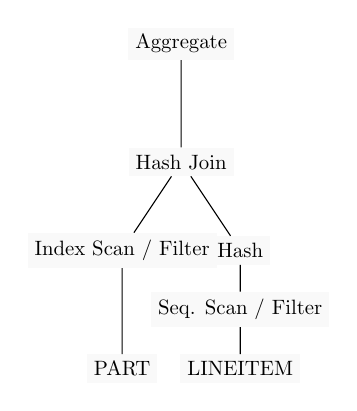
\begin{tikzpicture}[scale=.75, transform shape]

\tikzstyle{every node} = [rectangle, fill=gray!5]

\node (d) at (0,3.5) {Index Scan / Filter};
\node (c) at (0,1.5) {PART};

\node (s) at (2,3.5) {Hash};
\node (p) at (2,2.5) {Seq. Scan / Filter};
\node (a) at (2,1.5) {LINEITEM};

\node (e) at (1,5) {Hash Join};
\node (f) at (1,7)  {Aggregate};


\draw[-] (c) -- (d);
\draw[-] (a) -- (p);
\draw[-] (d) -- (e);
\draw[-] (p) -- (s);
\draw[-] (s) -- (e);
\draw[-] (e) -- (f);
\end{tikzpicture}
}

\caption{ Query execution plan trees}

\label{fig:plan_trees}

\end{figure*}




\subsection{Performance Metrics}
We measured the following performance metrics for each of the queries:
\begin{description}


\item [PCM Writes:] The total number of word (4B) updates that are applied to the PCM memory during
the query execution.
\item [CPU Cycles:] The total number of CPU cycles required to execute the query.
\item [Wear Distribution:] The frequency of writes measured on a per-256B-block basis.

\end{description}

\section{Experimental Results}
\label{sec:results}
Based on the above framework, we conducted a wide variety of experiments
and present a representative set of results here.  We begin by profiling the PCM Writes and CPU Cycles behavior of
the native and PCM-conscious executions for Q13, Q16 and Q19 --
these results are shown in Figure~\ref{fig:overall_results}.  In each of these figures, we provide both the total and
the break-ups on a per operator basis, with \emph{GB} and \emph{HJ} lables denoting Group-By and Hash Join operators, respectively.

\begin{figure*}[!h]

\centering

\subfloat[Impact of sort on overall performance - Q13]{
  \includegraphics[height=29mm]{overall_q13.png}
  
}
\hspace{0mm}
\subfloat[Impact of group-by on overall performance - Q16]{
  \includegraphics[height=29mm]{overall_q16.png}
}
\hspace{0mm}
\subfloat[Impact of hash join on overall performance - Q19]{
  \includegraphics[height=29mm]{overall_q19.png}
}
\caption{Overall performance of queries}
\label{fig:overall_results}
\end{figure*}


Focusing our attention first on Q13 in
Figure~\ref{fig:overall_results}(a), we find that the bulk of the
overall Writes and Cycles are consumed by the Sort operator. Comparing
the performance of the Native (blue bar) and PCM-conscious (green bar)
implementations, we observe a very significant savings (53\%) on Writes,
and an appreciable decrease (20\%) on Cycles.

Turning our attention to Q16 in Figure~\ref{fig:overall_results}(b),
we find that here it is the group-by operator that primarily influences
the overall Writes performance, whereas the hash-join determines the
Cycles behavior. Again, there are substantial savings in both Writes
(40\%) and  Cycles (30\%) delivered by the PCM-conscious approach.

Finally, moving on to Q19 in Figure~\ref{fig:overall_results}(c),
where hash-join is essentially the only operator, the
savings are around $64\%$ with regard to Writes and $32\%$ in Cycles.

\subsection{Operator-wise Analysis}
We now analyse the savings due to each operator independently and show
their correspondence to the analysis in Sections~\ref{sort}--\ref{gby} .

\paragraph{Sort.}
For Q13, as already mentioned, we observed savings of $53\%$ in writes and
$20\%$ in cycles.  In the case of Q16, the data at the sorting stage was
found to be much less than the DRAM size. Hence, both the native and
PCM-conscious executions used the standard sort routine, and as a result,
the cycles and writes for both implementations match exactly.

\paragraph{Hash Join.}
Each entry in the hash table consisted of a pointer to the build tuple
and a hash value field. New memory allocation to each bucket was done
in units of pages, with each page holding up to 64 entries. A search for
the matching join column began with the first tuple in the corresponding
bucket and went on till the last tuple in that bucket, simultaneously
writing out the join tuples for successful matches.  For Q16, we
observed a $12\%$ improvement in Writes and $31\%$ in Cycles due to the
PCM-conscious hash join, as shown in Figure~\ref{fig:overall_results}(b). The high savings in Cycles was the result of the caching effect due to page-wise allocation.
These improvements were even higher with Q19  -- 65\% Writes and 32\%
Cycles in Figure~\ref{fig:overall_results}(c) -- the source of the
enhancement was the 3 bytes of writes saved due to single-byte hash
values\footnote{The hash values of all entries within a bucket are placed contiguously.}, in addition to the page-based aggregation of hash table entries.


\paragraph{Group-By.}
In Q16, the aggregate operator in the group-by has an associated
\textit{distinct} clause.  Thus, our group-by algorithm utilized
hash-based in-place partitioning followed by sorting to carry out the
aggregation. Both the partitioning and sorting were carried out through
pointers, thereby reducing the writes significantly. Consequently,
we obtain savings of $74\%$ in Writes and $20\%$ in Cycles, as shown
in Figure~\ref{fig:overall_results}(b).  When we consider Q13, however,
the hash table consisted of very few entries. The less number of entries
led to the overhead of the page metadata construction overshadowing the
savings obtained in other aspects. Specifically, only marginal improvements
of about 4\% and 1\% were obtained for Writes and Cycles, as shown in
Figure~\ref{fig:overall_results}(a).

\begin{figure*}[t]
\centering

\subfloat[Q13]{
  \includegraphics[width=4cm]{wear_q13.png}
}
\subfloat[Q16]{
  \includegraphics[width=4cm]{wear_q16.png}
}
\subfloat[Q19]{
  \includegraphics[width=4cm]{wear_q19.png}
}
\caption{Queries wear distribution }
\label{fig:wear_dist}
\end{figure*}



\subsection{Lifetime Analysis}

The above experiments have shown that PCM-conscious operators
can certainly provide substantive improvements in both Writes and
Cycles. However, the question still remains as to whether these
improvements have been purchased at the expense of \emph{longevity} of
the memory. That is, are the writes skewed towards particular memory
locations?  To answer this, we show in Figure~\ref{fig:wear_dist}, the
maximum number of writes  across all memory blocks (as mentioned earlier,
we track writes at the block-level (256 bytes) in our modified simulator),
for the three TPC-H queries. The x-axis displays the block numbers in
decreasing order of writes.

We observe here that the maximum number of writes is considerably more for the
native systems as compared to the PCM-conscious processing. This
conclusively demonstrates that the improvement is with regard to
\emph{both} average-case and worst-case behavior.

\subsection{Validating Write Estimators}
\label{sec:validation}

We now move on to validating the estimators
(presented in Sections~\ref{sort} through \ref{gby})  for the number of
writes incurred by the various database operators.

\subsubsection{Sort}
The size of the $orders$ table is approximately $214 \times 10^6$ bytes. 
The flashsort algorithm incurred writes of $110.6 \times 10^6$ words $= 441.8 \times 10^6 $
bytes. Replacing the values for $N_R L_R$ with the table size in Equation \ref{eq:sort},
we get the writes as 
\begin{small}
$$W_{sort}(bytes) = 2 \times 214 \times
10^6  = 428 \times 10^6 $$ 
\end{small}
Thus the estimate is close to the observed writes.



\subsubsection{Hash Join}
For the hash join in Q19, the values of $N_R$, $size_{entry}$, $J$,
$size_{j}$ are $2 \times 10^5$, $5$ bytes, $120$ and $8$ bytes, respectively. 
Substituting the parameter values in Equation \ref{eq:hj}, the writes are given by:  
\begin{small}
$$W_{hj}(bytes) = 2 \times 10^5 \times 5 + 120 \times 8 \approx 10^6$$
\end{small}
which is close to the actual writes of $0.32 \times 10^6$ words $=
1.28 \times 10^6$ bytes.

  
\subsubsection{Group-By}
The values of the parameters $N_R$, $L_R$, $P$, $G$ and $size_g$ for Q16
are $119056$, $48$ bytes, $4$ bytes, $18341$ and $48$ bytes, respectively.  
The grouping algorithm used was sort-based grouping. Using Equation \ref{eq:gb_sort} results in:
\begin{small}
$$W_{gb\_sort}(bytes) = 2N_R \times P + G \times size_g = 2 \times 119056\times 4 + 18341 \times 48
= 1.83 \times 10^6$$
\end{small}
This closely corresponds to the observed writes of $0.36 \times 10^6$ words $= 1.44 \times 10^6$ bytes.

A summary of the above results is provided in
Table~\ref{tab:estimator_validation}. It is clear that our estimators
predict the write cardinality with an acceptable degree of accuracy for
the PCM-conscious implementations, making them suitable for incorporation
in the query optimizer.

\begin{table}[!h]                                                                                       
\centering                                                                                              
\caption{Validation of Write Estimators}
  \label{tab:estimator_validation}                                                                                
  %\centering                                                                                             
  \begin{small}                                                                                           
  \begin{tabular}{p{3cm}p{3cm}p{3cm}p{2.5cm}}
  \toprule                                                                                                
  
  \textbf{Operator} & \textbf{Estimated Writes} (e) & \textbf{Observed Writes} (o) & \textbf{Error Factor} $\frac{e-o}{o}$\\
  \midrule                                                                                                
  
    \textbf{Sort} &  $428 \times 10^6$ & $441.8 \times 10^6$ & -0.03\\ 
  \textbf{Hash Join} &  $1 \times 10^6$ & $1.28 \times 10^6$ & -0.22\\ 
  \textbf{Group-By} &  $1.83 \times 10^6$ &$1.44 \times 10^6$ & 0.27\\ 
  
  \bottomrule                                                                                             
  \end{tabular}                                                                                           
  \end{small}                                                                                             
  \end{table} 





